\section{Experimental Results}
\label{experiment}

\subsection{Dataset}
\label{experiment:dataset}
We experiment on trajectories data in four cities from \cite{ijcai15} that were
extracted from Yahoo! Flickr Creative Commons 100M (a.k.a. YFCC100M) dataset\cite{yfcc100m},
and trajectories data in Melbourne that was extracted from YFCC100M the same way described in \cite{ht10, ijcai15},
dataset statistics are available in table \ref{table:data:all}-\ref{table:data:perfect}.

An example of trajectory in Melbourne was shown in figure \ref{fig:traj}.

\begin{figure}
\centering
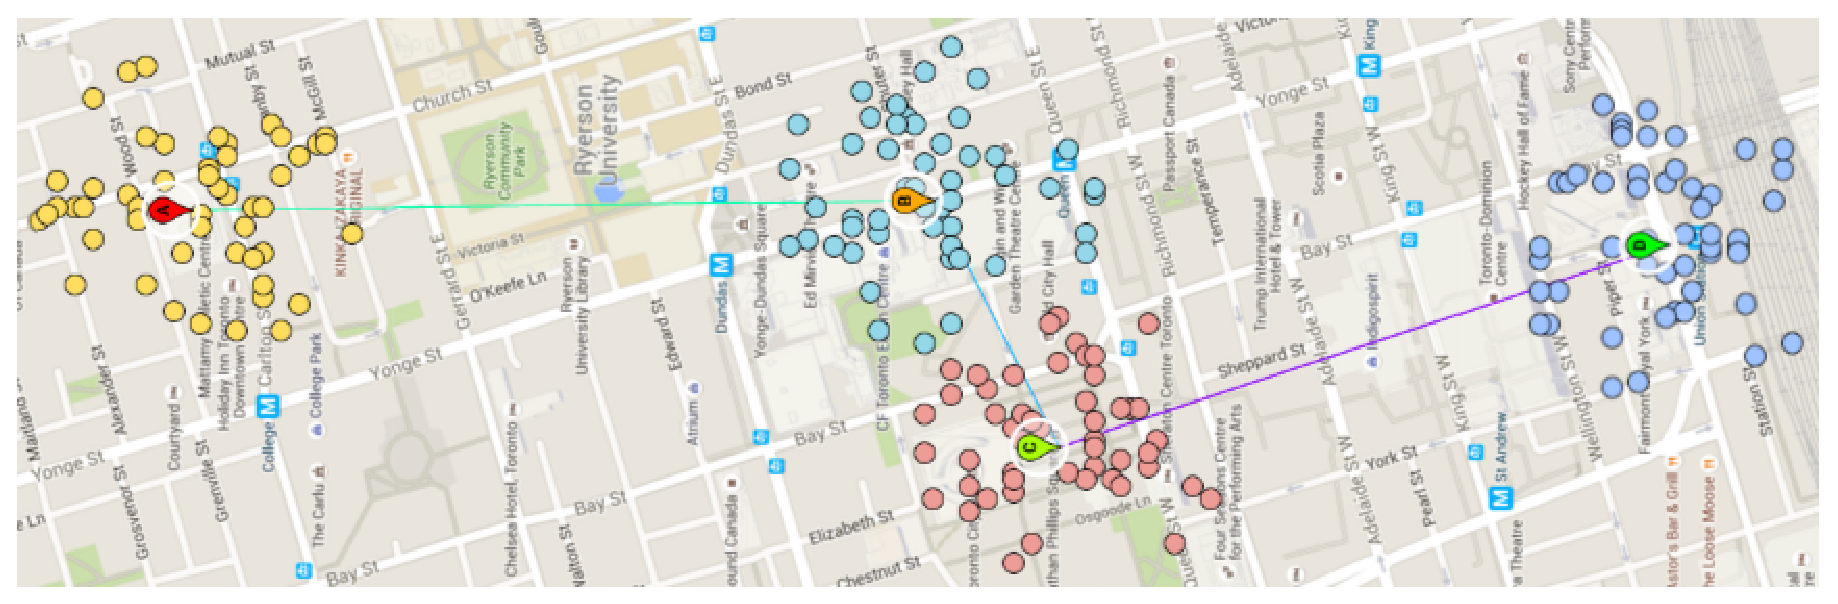
\epsfig{file=traj_eg.eps, width=3.5in}
\caption{An example of trajectory}
\label{fig:traj}
\end{figure}


\begin{table}
\centering
\caption{Dataset with all trajectories}
\label{table:data:all}
\scriptsize
\begin{tabular}{lrrrr} \hline
\textbf{City} & \textbf{\#POIs} & \textbf{\#Users} & \textbf{\#POI Visits} & \textbf{\#Trajectories} \\ \hline
Osaka & 27 & 450 & 7,747 & 1,115 \\ 
Glasgow & 27 & 601 & 11,434 & 2,227 \\ 
Edinburgh & 28 & 1,454 & 33,944 & 5,028 \\ 
Toronto & 29 & 1,395 & 39,419 & 6,057 \\ 
Melbourne & 85 & 832 & 23,794 & 4,918 \\ 
\hline
\end{tabular}
\end{table}

\begin{table}
\centering
\caption{Dataset without short trajectories}
\label{table:data:noshort}
\scriptsize
\begin{tabular}{lrrrr} \hline
\textbf{City} & \textbf{\#POIs} & \textbf{\#Users} & \textbf{\#POI Visits} & \textbf{\#Trajectories} \\ \hline
Osaka & 21 & 51 & 1,595 & 64 \\ 
Glasgow & 24 & 102 & 1,862 & 131 \\ 
Edinburgh & 26 & 423 & 13,136 & 710 \\ 
Toronto & 26 & 232 & 7,415 & 417 \\ 
Melbourne & 81 & 248 & 6,510 & 395 \\ 
\hline
\end{tabular}
\end{table}

\begin{table}
\centering
\caption{Dataset without trajectories that are short or with sub-tours}
\label{table:data:perfect}
\scriptsize
\begin{tabular}{lrrrr} \hline
\textbf{City} & \textbf{\#POIs} & \textbf{\#Users} & \textbf{\#POI Visits} & \textbf{\#Trajectories} \\ \hline
Osaka & 18 & 29 & 801 & 35 \\ 
Glasgow & 23 & 66 & 844 & 75 \\ 
Edinburgh & 26 & 249 & 4,570 & 365 \\ 
Toronto & 26 & 149 & 4,003 & 239 \\ 
Melbourne & 78 & 188 & 3,312 & 266 \\ 
\hline
\end{tabular}
\end{table}



\subsection{Evaluation Metrics}
\label{experiment:metric}
We use leave-one-out cross validation to evaluate different trajectory recommendation algorithms,
i.e., when evaluating a specific trajectory of a user, all other trajectories of this user as well as 
all trajectories of other users to train the recommendation algorithm.
Then employ trajectory F1-score defined in \cite{ijcai15} to compare the performance of different algorithms.


\subsection{Comparison}
% the way to binning POI features, #clusters of POIs,
\label{experiment:comparison}

We compared the experimental results on trajectory datasets between the proposed methods and other 7 methods:
\begin{itemize}
\item Random: choose POIs uniformly at random (without replacement) from the set of POIs $\mathcal{P} \setminus \{p_s, p_e \}$ to visit.
\item PersTour\cite{ijcai15}: personalised trajectory recommendation method described in \cite{ijcai15}, 
      time-based user interest was used and $\eta = 0.5$.
\item PersTour-L: PersTour\cite{ijcai15} with budget constraint replaced with the number POIs to visit, i.e., $L$,
      similar to PersTour, we use time-based user interest and set $\eta$ to $0.5$.
\item RankP: choose POIs according to the ranking based on POI popularity.
\item RankF: choose POIs according to the ranking based on POI features described in section \ref{method:ranking}.
\item MC-DP: recommend trajectory according to the Markov Chain with transition matrix described in section \ref{method:transition},
      use Viterbi algorithm to compute the most likely trajectory w.r.t. constraints $(p_s, p_e, L)$.
\item MC-ILP: the same as MC-DP, but use integer linear programming to compute the most likely trajectory.
\item Prop-DP: one of the proposed methods, combining POI ranking based on features 
      described in section \ref{method:ranking} and the Markov Chain with transition matrix described in section \ref{method:transition},
      use dynamic programming to compute the most likely trajectory w.r.t. constraints $(p_s, p_e, L)$.
\item Prop-ILP: the second proposed method, same as Prop-DP,
      but use integer linear programming to compute the most likely trajectory.
\end{itemize}

The regularisation parameter of rankSVM in RankF, Prop-DP and Prop-ILP was set to $1000$,
$K=100$ for user specific setting in RankF, RankP, MC-DP, MC-ILP, Prop-DP and Prop-ILP,
POI features used in MC-DP, MC-ILP, Prop-DP and Prop-ILP were discretized using parameters discribed in 
table \ref{table:discretize:all}-\ref{table:discretize:perfect}.


\begin{table}
\centering
\caption{POI Features Discretization Parameters: Dataset with all trajectories}
\label{table:discretize:all}
\scriptsize
\begin{tabular}{lcccc} \hline
\textbf{City} & \textbf{Popularity} & \textbf{\#Visits} & \textbf{Duration} & \textbf{Neighbourhood} \\ \hline
Osaka & 2 & 2 & 3 & 4 \\ 
Glasgow & 4 & 4 & 3 & 3 \\ 
Edinburgh & 4 & 3 & 3 & 3 \\ 
Toronto & 3 & 3 & 3 & 3 \\ 
Melbourne & 5 & 4 & 3 & 5 \\ 
\hline
\end{tabular}
\end{table}

\begin{table}
\centering
\caption{POI Features Discretization Parameters: Dataset without short trajectories}
\label{table:discretize:noshort}
\scriptsize
\begin{tabular}{lcccc} \hline
\textbf{City} & \textbf{Popularity} & \textbf{\#Visits} & \textbf{Duration} & \textbf{Neighbourhood} \\ \hline
Osaka & 3 & 3 & 5 & 4 \\ 
Glasgow & 3 & 4 & 5 & 4 \\ 
Edinburgh & 4 & 4 & 3 & 3 \\ 
Toronto & 2 & 4 & 3 & 3 \\ 
Melbourne & 3 & 2 & 5 & 3 \\ 
\hline
\end{tabular}
\end{table}

\begin{table}
\centering
\caption{POI Features Discretization Parameters: Dataset without trajectories that are short or with sub-tours}
\label{table:discretize:perfect}
\scriptsize
\begin{tabular}{lcccc} \hline
\textbf{City} & \textbf{Popularity} & \textbf{\#Visits} & \textbf{Duration} & \textbf{Neighbourhood} \\ \hline
Osaka & 2 & 2 & 3 & 4 \\ 
Glasgow & 2 & 2 & 3 & 4 \\ 
Edinburgh & 4 & 2 & 3 & 4 \\ 
Toronto & 3 & 3 & 3 & 3 \\ 
Melbourne & 5 & 5 & 4 & 3 \\ 
\hline
\end{tabular}
\end{table}


%\begin{tabular}{c|ccccccc|cccccccc} \hline
%\multirow{2}{*}{Dataset} & \multicolumn{7}{|c|}{User agnostic} & \multicolumn{8}{|c}{User specific} \\ \cline{2-15}
%                         & Rand & RankP & RankF & MC-DP & MC-ILP & Pro-DP & Pro-ILP 
%                         & PersTour & PersTour-L & RankP & RankF & MC-DP & MC-ILP & Pro-DP & Pro-ILP \\ \hline
%Toronto           & $1\pm0$ & $1\pm0$ & $1\pm0$ & $1\pm0$ & $1\pm0$ & $1\pm0$ & $1\pm0$ 
%                  & $1\pm0$ & $1\pm0$ & $1\pm0$ & $1\pm0$ & $1\pm0$ & $1\pm0$ & $\mathbf{1\pm0}$ & $1\pm0$ \\

\begin{table*}
    \centering
    \caption{Experimental Results: user agnostic setting with all trajectories}
    \begin{tabular}{l|ccccc} \hline
         & Osaka & Glasgow & Edinburgh & Toronto & Melbourne \\ \hline
        RankP & $0.611\pm0.163$ & $0.706\pm0.169$ & $\mathbf{0.644\pm0.169}$ & $0.638\pm0.141$ & $0.563\pm0.140$ \\
        RankF & $0.633\pm0.153$ & $\mathbf{0.758\pm0.182}$ & $0.634\pm0.153$ & $\mathbf{0.707\pm0.178}$ & $0.570\pm0.134$ \\
        MC-DP & $0.707\pm0.229$ & $0.695\pm0.180$ & $0.560\pm0.175$ & $0.637\pm0.170$ & $0.518\pm0.166$ \\
        MC-ILP & $0.670\pm0.209$ & $0.696\pm0.166$ & $0.594\pm0.136$ & $0.652\pm0.149$ & $0.534\pm0.148$ \\
        Prop-DP & $\mathbf{0.709\pm0.202}$ & $0.706\pm0.175$ & $0.611\pm0.182$ & $0.684\pm0.195$ & $0.552\pm0.179$ \\
        Prop-ILP & $0.660\pm0.206$ & $0.711\pm0.170$ & $0.626\pm0.152$ & $0.701\pm0.176$ & $\mathbf{0.579\pm0.156}$ \\
        \hline
    \end{tabular}
\end{table*}

\begin{table*}
    \centering
    \caption{Experimental Results: user specific setting with all trajectories}
    \begin{tabular}{l|ccccc} \hline
         & Osaka & Glasgow & Edinburgh & Toronto & Melbourne \\ \hline
        RankP & $0.611\pm0.163$ & $0.706\pm0.169$ & $\mathbf{0.644\pm0.169}$ & $0.638\pm0.141$ & $0.563\pm0.140$ \\
        RankF & $0.647\pm0.170$ & $\mathbf{0.754\pm0.179}$ & $0.635\pm0.155$ & $\mathbf{0.708\pm0.178}$ & $0.569\pm0.134$ \\
        MC-DP & $\mathbf{0.706\pm0.218}$ & $0.689\pm0.181$ & $0.561\pm0.181$ & $0.640\pm0.175$ & $0.537\pm0.177$ \\
        MC-ILP & $0.656\pm0.198$ & $0.696\pm0.177$ & $0.598\pm0.152$ & $0.661\pm0.156$ & $0.552\pm0.162$ \\
        Prop-DP & $0.658\pm0.192$ & $0.700\pm0.169$ & $0.614\pm0.185$ & $0.691\pm0.196$ & $0.563\pm0.166$ \\
        Prop-ILP & $0.635\pm0.190$ & $0.705\pm0.163$ & $0.628\pm0.154$ & $0.702\pm0.178$ & $\mathbf{0.578\pm0.157}$ \\
        \hline
    \end{tabular}
\end{table*}

\begin{table*}
    \centering
    \caption{Experimental Results: user agnostic setting without short trajectories}
    \begin{tabular}{l|ccccc} \hline
         & Osaka & Glasgow & Edinburgh & Toronto & Melbourne \\ \hline
        RankP & $0.630\pm0.175$ & $0.705\pm0.171$ & $0.641\pm0.163$ & $0.653\pm0.145$ & $0.570\pm0.141$ \\
        RankF & $0.639\pm0.182$ & $\mathbf{0.749\pm0.174}$ & $\mathbf{0.644\pm0.162}$ & $\mathbf{0.713\pm0.178}$ & $0.573\pm0.138$ \\
        MC-DP & $0.690\pm0.205$ & $0.718\pm0.188$ & $0.564\pm0.191$ & $0.687\pm0.185$ & $0.525\pm0.173$ \\
        MC-ILP & $0.651\pm0.194$ & $0.716\pm0.186$ & $0.595\pm0.157$ & $0.687\pm0.167$ & $0.547\pm0.150$ \\
        Prop-DP & $\mathbf{0.717\pm0.215}$ & $0.734\pm0.183$ & $0.615\pm0.196$ & $0.681\pm0.197$ & $0.548\pm0.175$ \\
        Prop-ILP & $0.691\pm0.196$ & $0.736\pm0.175$ & $0.625\pm0.161$ & $0.703\pm0.166$ & $\mathbf{0.576\pm0.157}$ \\
        \hline
    \end{tabular}
\end{table*}

\begin{table*}
    \centering
    \caption{Experimental Results: user specific setting without short trajectories}
    \begin{tabular}{l|ccccc} \hline
         & Osaka & Glasgow & Edinburgh & Toronto & Melbourne \\ \hline
        RankP & $0.630\pm0.175$ & $0.705\pm0.171$ & $0.641\pm0.163$ & $0.653\pm0.145$ & $0.570\pm0.141$ \\
        RankF & $0.648\pm0.202$ & $\mathbf{0.742\pm0.171}$ & $\mathbf{0.643\pm0.162}$ & $\mathbf{0.715\pm0.178}$ & $0.570\pm0.137$ \\
        MC-DP & $0.674\pm0.179$ & $0.707\pm0.179$ & $0.575\pm0.196$ & $0.685\pm0.181$ & $0.535\pm0.170$ \\
        MC-ILP & $0.630\pm0.171$ & $0.712\pm0.173$ & $0.602\pm0.164$ & $0.690\pm0.164$ & $0.555\pm0.152$ \\
        Prop-DP & $\mathbf{0.714\pm0.207}$ & $0.728\pm0.179$ & $0.616\pm0.196$ & $0.693\pm0.186$ & $0.560\pm0.174$ \\
        Prop-ILP & $0.681\pm0.194$ & $0.735\pm0.172$ & $0.625\pm0.162$ & $0.705\pm0.169$ & $\mathbf{0.575\pm0.160}$ \\
        \hline
    \end{tabular}
\end{table*}

\subsection{Analysis of Experimental Results}
\label{experiment:analysis}
